\documentclass[11pt,aspectratio=169]{beamer}

\usetheme{Madrid}
\definecolor{navy}{HTML}{1F3A68}
\definecolor{gold}{HTML}{C9A227}
\setbeamercolor{structure}{fg=navy}
\setbeamercolor{palette primary}{bg=navy,fg=white}
\setbeamercolor{palette secondary}{bg=navy!85,fg=white}
\setbeamercolor{palette tertiary}{bg=navy!70,fg=white}
\setbeamercolor{frametitle}{bg=navy,fg=white}
\setbeamercolor{title}{bg=navy,fg=white}
\setbeamercolor{block title}{bg=navy,fg=white}
\setbeamercolor{block body}{bg=navy!6}
\setbeamertemplate{navigation symbols}{}
\setbeamertemplate{bibliography item}[text]

\usepackage{amsmath,amssymb}
\usepackage{bm}
\usepackage{booktabs}
\usepackage{tabularx}
\usepackage{graphicx}
\usepackage{multirow}
\usepackage{algorithm}
\usepackage{algpseudocode}
\usepackage{tikz}

% Shared assets produced by `python main.py --export-latex` (see code/README.md).
\graphicspath{{../shared/figures/}}
% AUTO-GENERATED by code/main.py --export-latex. Do not edit; re-run the export instead.
\newcommand{\NumVertices}{10}
\newcommand{\NumEdges}{45}
\newcommand{\StartName}{USTP Cagayan de Oro Campus}
\newcommand{\DCSeed}{1}
\newcommand{\DCRule}{bridge}
\newcommand{\DCRoute}{V0 $\to$ V1 $\to$ V7 $\to$ V9 $\to$ V2 $\to$ V3 $\to$ V4 $\to$ V5 $\to$ V6 $\to$ V8 $\to$ V0}
\newcommand{\DCTotal}{13.82}
\newcommand{\DCRecomputed}{13.82}
\newcommand{\DCAllChecks}{passed}
\newcommand{\OptRoute}{V0 $\to$ V8 $\to$ V6 $\to$ V4 $\to$ V5 $\to$ V3 $\to$ V2 $\to$ V9 $\to$ V7 $\to$ V1 $\to$ V0}
\newcommand{\OptTotal}{13.61}
\newcommand{\DCGap}{1.54}
\newcommand{\RunCount}{100}
\newcommand{\BridgeMean}{13.88}
\newcommand{\BridgeBest}{13.61}
\newcommand{\BridgeWorst}{14.26}
\newcommand{\BridgeMeanGap}{2.01}
\newcommand{\BridgeOptHits}{6}
\newcommand{\BestRuleOptHits}{17}
\newcommand{\BestRuleMean}{13.91}
\newcommand{\BestRuleBest}{13.61}
\newcommand{\BestRuleWorst}{14.13}
\newcommand{\BestRuleMeanGap}{2.20}


% Red reminder for things the group still has to fill in or confirm. Remove before presenting.
\newcommand{\groupnote}[1]{\textcolor{red}{[#1]}}

\title[Divide \& Conquer for TSP]{Divide and Conquer for the\\Traveling Salesperson Problem}
\subtitle{A One-Day City Tour of Downtown Cagayan de Oro}
\author[Chiong, Limpahan, Locsin, Sajol]{Heart Chiong \and Mark Vincent Limpahan \and Roxanne Locsin \and Rhenel Jhon Sajol}
\institute[Graph Theory PIT]{Graph Theory --- Performance Innovative Task (Algorithm 2.8)}
\date{October 18, 2026\\CS414 Graph Theory\\Instructor: Dr. Penelyn L. Acal}

\begin{document}

\begin{frame}
  \titlepage
\end{frame}

\begin{frame}{Outline}
  \tableofcontents
\end{frame}

% Suggested time: 2-3 minutes
\section{Problem and Objective}

\begin{frame}{The Traveling Salesperson Problem}
  \begin{itemize}
    \item Visit every required location \textbf{exactly once} and \textbf{return to the start},
          with the smallest total cost.
    \item In graph terms: find a \textbf{minimum-weight Hamiltonian cycle}.
    \item NP-hard~\cite{garey1979computers}: exact methods blow up
          (brute force $O(n!)$, Held--Karp $O(n^2 2^n)$).
    \item So we use fast \textbf{heuristics}. Ours is \textbf{Divide and Conquer}, Algorithm~2.8 of
          Luna-Garcia, Candano \& Caga-anan (2024)~\cite{lunagarcia2024performance}.
  \end{itemize}
\end{frame}

\begin{frame}{Our Real-Life Problem: A Downtown Cagayan de Oro Tour}
  \begin{columns}[T]
    \begin{column}{0.55\textwidth}
      \textbf{Situation.} The university hosts visiting guests and takes them on a one-day tour by
      service vehicle.
      \medskip

      \textbf{Start / end:} V0 --- \StartName.

      \textbf{Required stops:} 9 downtown landmarks (V1--V9), all within about $2.5\times2$ km.
      \medskip

      \textbf{Objective:} minimise the total \textbf{driving distance (km)}
      \[ L(T) = \sum_{k=0}^{n-1} w(v_k, v_{k+1}),\quad v_0 = v_n = \mathrm{V0}. \]
    \end{column}
    \begin{column}{0.42\textwidth}
      \begin{block}{Assumptions}
        \small
        \begin{itemize}
          \item Car; shortest driving route between stops
          \item Distance the same both ways
          \item No traffic, opening hours or dwell time
        \end{itemize}
      \end{block}
      \begin{block}{Constraints}
        \small
        \begin{itemize}
          \item Start and end at V0
          \item Each stop visited exactly once
        \end{itemize}
      \end{block}
    \end{column}
  \end{columns}
\end{frame}

% Suggested time: 2-3 minutes
\section{The Divide and Conquer Algorithm}

\begin{frame}{Divide and Conquer: The Procedure}
  \begin{columns}[T]
    \begin{column}{0.56\textwidth}
      \small
      \begin{enumerate}
        \item \textbf{Shuffle} the cities at random.
        \item \textbf{Divide:} pick the $x$ or $y$ axis at random, sort, and cut at the median.
        \item \textbf{Base cases:} 1 city $\Rightarrow$ length 0; \\
              2 cities $a,b$ $\Rightarrow$ tour $a\to b\to a$, length $2w(a,b)$.
        \item \textbf{Conquer:} solve both halves recursively.
        \item \textbf{Combine:} join the two tours through the \textbf{shortest bridge}.
        \item \textbf{Adjust} so that no city repeats.
      \end{enumerate}
    \end{column}
    \begin{column}{0.42\textwidth}
      \begin{block}{Complexity}
        \[ T(n) = 2T(n/2) + \underbrace{O(n^2)}_{\text{bridge search}} = O(n^2) \]
        \small Merge cost halves at each level: a geometric series~\cite{cormen2009introduction}.
      \end{block}
    \end{column}
  \end{columns}
\end{frame}

\begin{frame}{The Merge Step (and a Fix to the Paper's Code)}
  \begin{columns}[T]
    \begin{column}{0.5\textwidth}
      \small
      \textbf{Paper's code:} \texttt{tour1[:-1] + [a,b] + tour2}
      \begin{itemize}
        \item The bridge cities $a, b$ end up \textbf{repeated}.
        \item On the paper's 7-city example it returns 13 entries and does not return to the start.
      \end{itemize}
      \medskip
      \textbf{Our merge (keeps the shortest bridge):}
      \begin{enumerate}
        \item Find the shortest bridge $(a,b)$.
        \item Remove one edge $(a,a')$ of $T_1$ and one edge $(b,b')$ of $T_2$.
        \item Add $(a,b)$ and $(a',b')$; keep the cheapest choice:
      \end{enumerate}
      \[ \Delta = w(a,b) + w(a',b') - w(a,a') - w(b,b') \]
    \end{column}
    \begin{column}{0.48\textwidth}
      \centering
      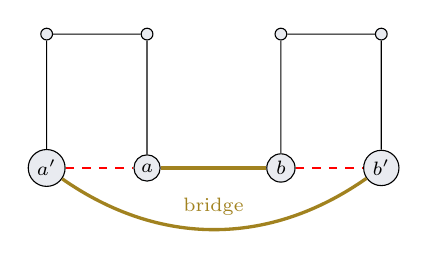
\begin{tikzpicture}[scale=0.85, every node/.style={circle, draw, fill=navy!10, inner sep=1.5pt, font=\scriptsize}]
        \node (a1) at (0,0) {$a'$}; \node (a) at (1.5,0) {$a$};
        \node (c1) at (1.5,2) {}; \node (c2) at (0,2) {};
        \node (b) at (3.5,0) {$b$}; \node (b1) at (5,0) {$b'$};
        \node (d1) at (5,2) {}; \node (d2) at (3.5,2) {};
        \draw (a) -- (c1) -- (c2) -- (a1);
        \draw[dashed, red] (a1) -- (a);
        \draw (b) -- (d2) -- (d1) -- (b1);
        \draw[dashed, red] (b) -- (b1);
        \draw[very thick, gold!80!black] (a) -- node[draw=none, fill=none, below] {bridge} (b);
        \draw[very thick, gold!80!black] (a1) to[bend right=35] (b1);
      \end{tikzpicture}

      \scriptsize \textcolor{red}{dashed} = removed, \textcolor{gold!80!black}{gold} = added. \\
      Result: one cycle, every city exactly once.
    \end{column}
  \end{columns}
\end{frame}

\begin{frame}{Advantages, Limitations, Optimality}
  \begin{columns}[T]
    \begin{column}{0.48\textwidth}
      \begin{block}{Advantages}
        \small
        \begin{itemize}
          \item Fast: $O(n^2)$
          \item Simple; halves can run in parallel
          \item Nearby places tend to be visited together
        \end{itemize}
      \end{block}
    \end{column}
    \begin{column}{0.48\textwidth}
      \begin{block}{Limitations}
        \small
        \begin{itemize}
          \item Greedy merges are never undone
          \item Result depends on the random splits
          \item Splits by map position, not road distance
          \item Weakest average quality in the paper at 128--256 cities~\cite{lunagarcia2024performance}
        \end{itemize}
      \end{block}
    \end{column}
  \end{columns}
  \bigskip
  \begin{center}
    \textbf{Heuristic:} always a valid tour, \textbf{no guarantee of optimality}.
  \end{center}
\end{frame}

% Suggested time: 2-3 minutes
\section{Graph Model and Data}

\begin{frame}{Vertices: \NumVertices{} Locations in Cagayan de Oro}
  \centering
  \scriptsize
  \renewcommand{\arraystretch}{0.92}
  % AUTO-GENERATED by code/main.py --export-latex. Do not edit; re-run the export instead.
\begin{tabular}{l l l r r}
\toprule
\textbf{Vertex} & \textbf{Location} & \textbf{Area} & \textbf{Latitude} & \textbf{Longitude} \\
\midrule
V0 & USTP Cagayan de Oro Campus (start) & C. M. Recto Ave, Lapasan & 8.48607 & 124.65681 \\
V1 & Limketkai Center & Lapasan & 8.48139 & 124.65637 \\
V2 & Centrio Mall & C. M. Recto Ave, Licoan & 8.48483 & 124.65062 \\
V3 & Pelaez Sports Center & Don Apolinar Velez St, Burgos & 8.48180 & 124.64702 \\
V4 & Museo de Oro (Xavier University) & Corrales Ave, Nazareth & 8.47587 & 124.64598 \\
V5 & Divisoria Plaza & Barangay 5, Carmen & 8.47750 & 124.64465 \\
V6 & St. Augustine Metropolitan Cathedral & Gaston Circle, Carmen & 8.47497 & 124.64147 \\
V7 & Port of Cagayan de Oro & Macabalan & 8.49453 & 124.66219 \\
V8 & Liceo de Cagayan University & R. N. Pelaez Blvd, Carmen & 8.48566 & 124.63927 \\
V9 & Capitol University & Corrales Ext, Barangay 25 & 8.48818 & 124.65257 \\
\bottomrule
\end{tabular}

  \medskip
  \raggedright\footnotesize
  Coordinates: OpenStreetMap / Nominatim~\cite{osm}, located on Google Maps~\cite{googlemaps}.
\end{frame}

\begin{frame}{The Weighted Graph $G = K_{\NumVertices}$}
  \centering
  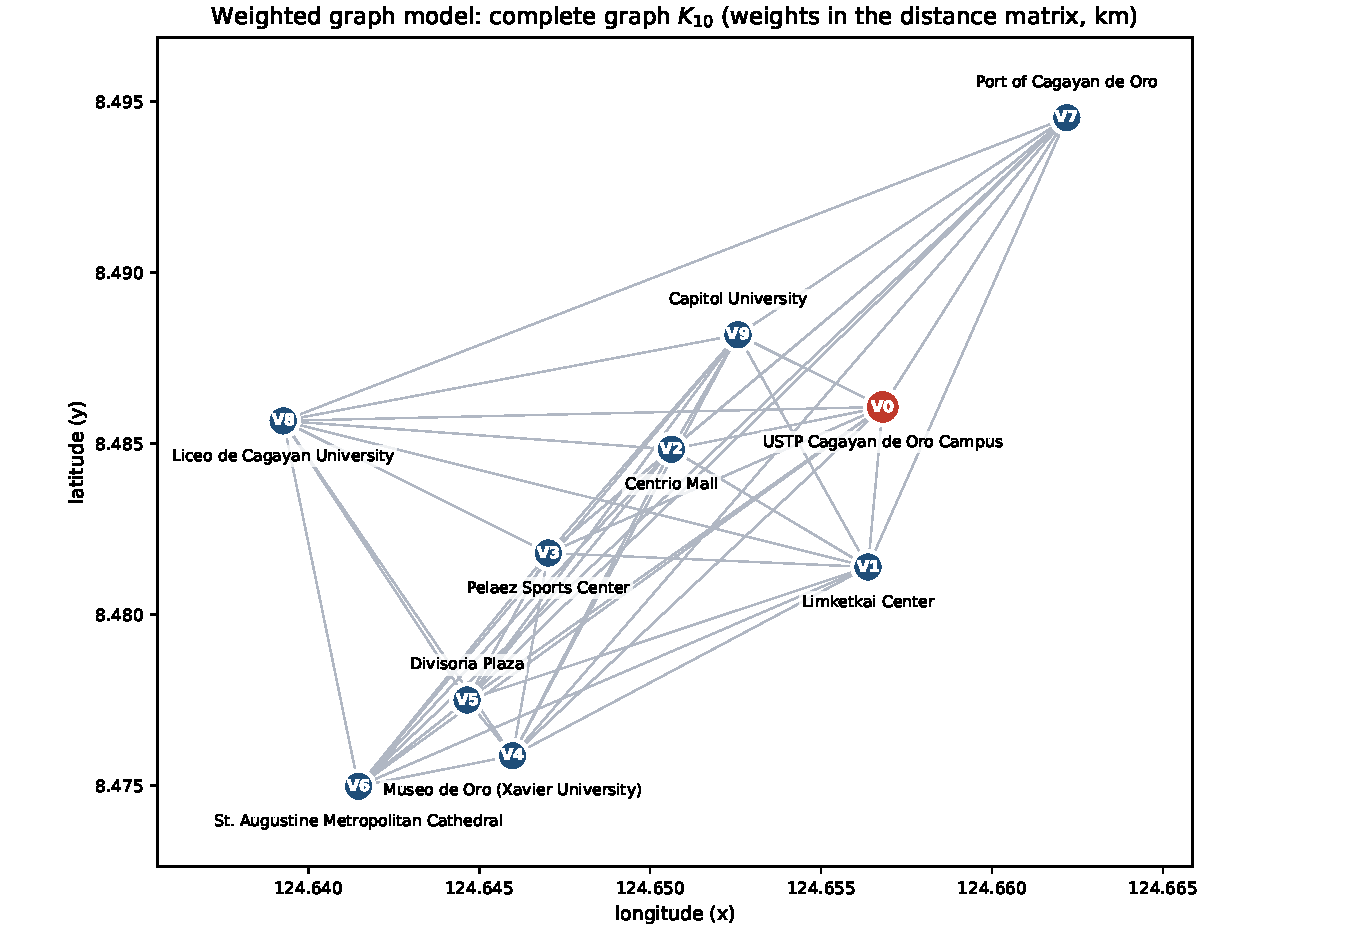
\includegraphics[height=0.78\textheight]{graph.pdf}

  \footnotesize Complete graph: \NumEdges{} edges, one for each pair of locations; each edge is the
  driving route OSRM returns between them (it may pass other stops without visiting them).
\end{frame}

\begin{frame}{Edges, Direction and Weights}
  \begin{columns}[T]
    \begin{column}{0.62\textwidth}
      \centering
      \resizebox{\linewidth}{!}{% AUTO-GENERATED by code/main.py --export-latex. Do not edit; re-run the export instead.
\begin{tabular}{l rrrrrrrrrr}
\toprule
 & \textbf{V0} & \textbf{V1} & \textbf{V2} & \textbf{V3} & \textbf{V4} & \textbf{V5} & \textbf{V6} & \textbf{V7} & \textbf{V8} & \textbf{V9} \\
\midrule
\textbf{V0} & -- & 1.09 & 1.26 & 1.94 & 2.48 & 2.37 & 2.83 & 2.07 & 2.62 & 1.34 \\
\textbf{V1} & 1.09 & -- & 1.55 & 2.24 & 2.10 & 2.21 & 2.50 & 2.32 & 2.96 & 1.68 \\
\textbf{V2} & 1.26 & 1.55 & -- & 1.18 & 1.55 & 1.61 & 1.85 & 2.17 & 1.86 & 0.58 \\
\textbf{V3} & 1.94 & 2.24 & 1.18 & -- & 1.31 & 0.97 & 1.43 & 2.98 & 2.15 & 1.38 \\
\textbf{V4} & 2.48 & 2.10 & 1.55 & 1.31 & -- & 0.54 & 0.87 & 3.52 & 1.92 & 1.93 \\
\textbf{V5} & 2.37 & 2.21 & 1.61 & 0.97 & 0.54 & -- & 0.74 & 3.29 & 1.58 & 1.70 \\
\textbf{V6} & 2.83 & 2.50 & 1.85 & 1.43 & 0.87 & 0.74 & -- & 3.87 & 1.65 & 2.28 \\
\textbf{V7} & 2.07 & 2.32 & 2.17 & 2.98 & 3.52 & 3.29 & 3.87 & -- & 3.66 & 1.79 \\
\textbf{V8} & 2.62 & 2.96 & 1.86 & 2.15 & 1.92 & 1.58 & 1.65 & 3.66 & -- & 2.06 \\
\textbf{V9} & 1.34 & 1.68 & 0.58 & 1.38 & 1.93 & 1.70 & 2.28 & 1.79 & 2.06 & -- \\
\bottomrule
\end{tabular}
}

      \scriptsize $w(i,j)$ = road distance in \textbf{km}
    \end{column}
    \begin{column}{0.36\textwidth}
      \footnotesize
      \textbf{Undirected:} one-way streets make raw distances differ slightly, so
      \[ w(u,v) = \tfrac12\bigl(d(u{\to}v) + d(v{\to}u)\bigr) \]
      \textbf{Actual data:} locations; road distances from the OSRM Table service~\cite{osrmapi}
      on the OpenStreetMap road network~\cite{luxen2011osrm}.

      \textbf{Assumed:} symmetric averaging; no traffic or time windows; choice of stops.
    \end{column}
  \end{columns}
\end{frame}

\begin{frame}{Cross-Check with Google Maps}
  \begin{columns}[T]
    \begin{column}{0.55\textwidth}
      \centering
      \scriptsize
      \setlength{\tabcolsep}{4pt}
      \begin{tabular}{c l r r r}
        \toprule
        \textbf{Leg} & \textbf{From $\to$ To} & \textbf{Matrix} & \textbf{Google} & \textbf{\%} \\
        \midrule
        1 & V0 $\to$ V1 & 1.09 & 0.70 & $-36$ \\
        2 & V1 $\to$ V7 & 2.32 & 3.10 & $+34$ \\
        3 & V7 $\to$ V9 & 1.79 & 2.00 & $+12$ \\
        4 & V9 $\to$ V2 & 0.58 & 0.65 & $+12$ \\
        5 & V2 $\to$ V3 & 1.18 & 1.10 & $-7$ \\
        6 & V3 $\to$ V4 & 1.31 & 1.70 & $+30$ \\
        7 & V4 $\to$ V5 & 0.54 & 0.70 & $+30$ \\
        8 & V5 $\to$ V6 & 0.74 & 0.45 & $-39$ \\
        9 & V6 $\to$ V8 & 1.65 & 1.60 & $-3$ \\
        10 & V8 $\to$ V0 & 2.62 & 2.40 & $-8$ \\
        \midrule
        & \textbf{Total} & \textbf{13.82} & \textbf{14.40} & $+4.2$ \\
        \bottomrule
      \end{tabular}
    \end{column}
    \begin{column}{0.42\textwidth}
      \footnotesize
      Each leg of our route searched separately on Google Maps~\cite{googlemaps} in driving mode.
      \medskip

      \textbf{Whole tour:} within \textbf{4.2\%}.

      \textbf{Single legs:} differ by up to 39\% (pin positions, one-way streets, different road
      choices and turn restrictions).
      \medskip

      We keep the OSRM matrix: it is reproducible and read directly by the program.
    \end{column}
  \end{columns}
\end{frame}

\begin{frame}{Applying the Algorithm: Divide (seed \DCSeed{})}
  \centering
  \resizebox{0.95\textwidth}{!}{% AUTO-GENERATED by code/main.py --export-latex. Do not edit; re-run the export instead.
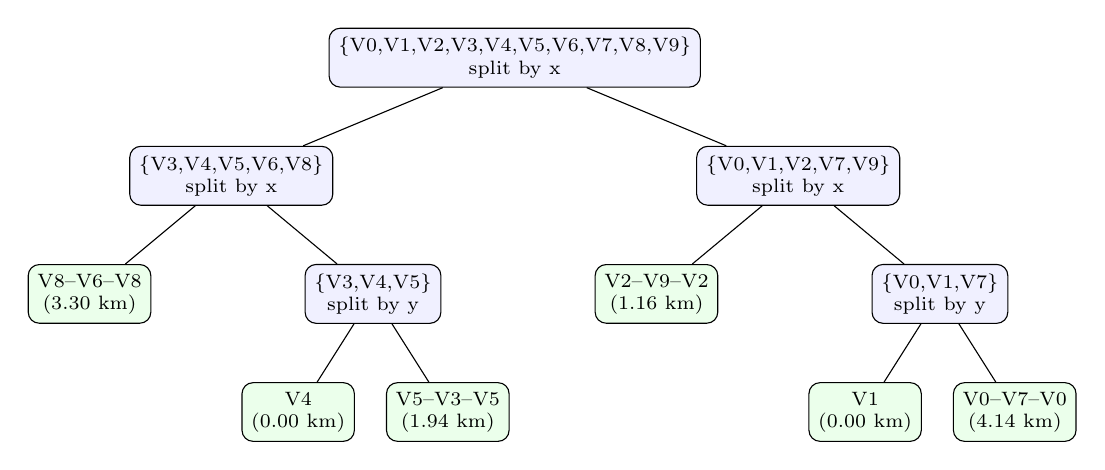
\begin{tikzpicture}[
  split/.style={draw, rounded corners, fill=blue!6, align=center, font=\scriptsize},
  leaf/.style={draw, rounded corners, fill=green!8, align=center, font=\scriptsize},
  level 1/.style={sibling distance=7.2cm, level distance=1.5cm},
  level 2/.style={sibling distance=3.6cm, level distance=1.5cm},
  level 3/.style={sibling distance=1.9cm, level distance=1.5cm}]
\node[split] {\{V0,V1,V2,V3,V4,V5,V6,V7,V8,V9\}\\split by x}
  child {
    node[split] {\{V3,V4,V5,V6,V8\}\\split by x}
    child {
      node[leaf] {V8--\allowbreak V6--\allowbreak V8\\(3.30 km)}
    }
    child {
      node[split] {\{V3,V4,V5\}\\split by y}
      child {
        node[leaf] {V4\\(0.00 km)}
      }
      child {
        node[leaf] {V5--\allowbreak V3--\allowbreak V5\\(1.94 km)}
      }
    }
  }
  child {
    node[split] {\{V0,V1,V2,V7,V9\}\\split by x}
    child {
      node[leaf] {V2--\allowbreak V9--\allowbreak V2\\(1.16 km)}
    }
    child {
      node[split] {\{V0,V1,V7\}\\split by y}
      child {
        node[leaf] {V1\\(0.00 km)}
      }
      child {
        node[leaf] {V0--\allowbreak V7--\allowbreak V0\\(4.14 km)}
      }
    }
  };
\end{tikzpicture}
}

  \footnotesize $x$ = longitude, $y$ = latitude. Leaves are the base-case tours.
\end{frame}

\begin{frame}{Applying the Algorithm: Conquer and Combine}
  \centering
  \tiny
  \setlength{\tabcolsep}{2.5pt}
  \resizebox{\textwidth}{!}{% AUTO-GENERATED by code/main.py --export-latex. Do not edit; re-run the export instead.
\begin{tabular}{c >{\raggedright\arraybackslash}p{2.6cm} >{\raggedright\arraybackslash}p{2.6cm} >{\raggedright\arraybackslash}p{1.9cm} >{\raggedright\arraybackslash}p{2.45cm} >{\raggedright\arraybackslash}p{2.45cm} r r}
\toprule
\textbf{Step} & \textbf{Left tour (km)} & \textbf{Right tour (km)} & \textbf{Shortest bridge} & \textbf{Edges removed} & \textbf{Edges added} & $\boldsymbol{\Delta}$ & \textbf{Merged} \\
\midrule
M1 & V4 (0.00) & V5--\allowbreak V3--\allowbreak V5 (1.94) & V4--V5 (0.54) & V5--V3 (0.97) & V4--V3 (1.31), V5--V4 (0.54) & +0.88 & 2.82 \\
M2 & V8--\allowbreak V6--\allowbreak V8 (3.30) & V4--\allowbreak V3--\allowbreak V5--\allowbreak V4 (2.82) & V6--V5 (0.74) & V8--V6 (1.65), V3--V5 (0.97) & V8--V3 (2.15), V5--V6 (0.74) & +0.27 & 6.39 \\
M3 & V1 (0.00) & V0--\allowbreak V7--\allowbreak V0 (4.14) & V1--V0 (1.09) & V0--V7 (2.07) & V1--V7 (2.32), V0--V1 (1.09) & +1.34 & 5.48 \\
M4 & V2--\allowbreak V9--\allowbreak V2 (1.16) & V1--\allowbreak V7--\allowbreak V0--\allowbreak V1 (5.48) & V2--V0 (1.26) & V2--V9 (0.58), V7--V0 (2.07) & V2--V0 (1.26), V7--V9 (1.79) & +0.40 & 7.04 \\
M5 & V6--\allowbreak V8--\allowbreak V3--\allowbreak V4--\allowbreak V5--\allowbreak V6 (6.39) & V9--\allowbreak V2--\allowbreak V0--\allowbreak V1--\allowbreak V7--\allowbreak V9 (7.04) & V3--V2 (1.18) & V8--V3 (2.15), V2--V0 (1.26) & V8--V0 (2.62), V2--V3 (1.18) & +0.39 & 13.82 \\
\bottomrule
\end{tabular}
}

  \medskip
  \footnotesize Each row: $L(T) = L(T_1) + L(T_2) + \Delta$ \quad (weights in km)
\end{frame}

\begin{frame}{Worked Calculation: the Final Merge}
  \small
  % AUTO-GENERATED by code/main.py --export-latex. Do not edit; re-run the export instead.
The two halves return the sub-tours $T_1 = $ V6--\allowbreak V8--\allowbreak V3--\allowbreak V4--\allowbreak V5--\allowbreak V6 (length 6.39 km) and $T_2 = $ V9--\allowbreak V2--\allowbreak V0--\allowbreak V1--\allowbreak V7--\allowbreak V9 (length 7.04 km).
Checking all $|T_1|\cdot|T_2| = 5\cdot5 = 25$ cross pairs, the shortest bridge is V3--V2 with $w = 1.18$ km.
Among the ways of opening one edge next to each bridge endpoint and closing the loop, the cheapest removes V8--V3 and V2--V0 and adds V8--V0 and V2--V3:
\[\Delta = (2.62 + 1.18) - (2.15 + 1.26) = +0.39\text{ km},\]
\[L(T) = L(T_1) + L(T_2) + \Delta = 6.39 + 7.04 + 0.39 = 13.82\text{ km}.\]
The merged cycle is V3--\allowbreak V4--\allowbreak V5--\allowbreak V6--\allowbreak V8--\allowbreak V0--\allowbreak V1--\allowbreak V7--\allowbreak V9--\allowbreak V2--\allowbreak V3, which visits all 10 vertices once.

\end{frame}

% Suggested time: 3-4 minutes (includes the live screen recording)
\section{Python Implementation and Results}

\begin{frame}{Code Components}
  \small
  \begin{tabularx}{\textwidth}{l >{\raggedright\arraybackslash}X}
    \toprule
    \textbf{Code} & \textbf{What it does} \\
    \midrule
    \texttt{data/*.csv} & Input: vertices (\texttt{locations.csv}) and weights (\texttt{distance\_matrix\_km.csv}) \\
    \texttt{split} & Divide: random axis, sort, median cut \\
    \texttt{solve} & Recursion and base cases; records each step \\
    \texttt{shortest\_bridge}, \texttt{merge} & Combine: bridge, remove 2 edges, add 2, smallest $\Delta$ \\
    \texttt{check\_route} & Valid closed tour? Recompute the total from the weights \\
    \texttt{held\_karp} & Exact optimum, \emph{for comparison only} \\
    \bottomrule
  \end{tabularx}
\end{frame}

\begin{frame}{Live Demo}
  \centering
  \Large\texttt{python main.py}
  \bigskip

  \normalsize
  \begin{enumerate}
    \item Input data: vertices and weight matrix
    \item Every divide, base-case and merge step, with its arithmetic
    \item Resulting route and total distance
    \item Verification checks
    \item Comparison with the exact optimum
  \end{enumerate}
  \bigskip
  \groupnote{Switch to the screen recording here}
\end{frame}

\begin{frame}{Resulting Route: \DCTotal{} km}
  \centering
  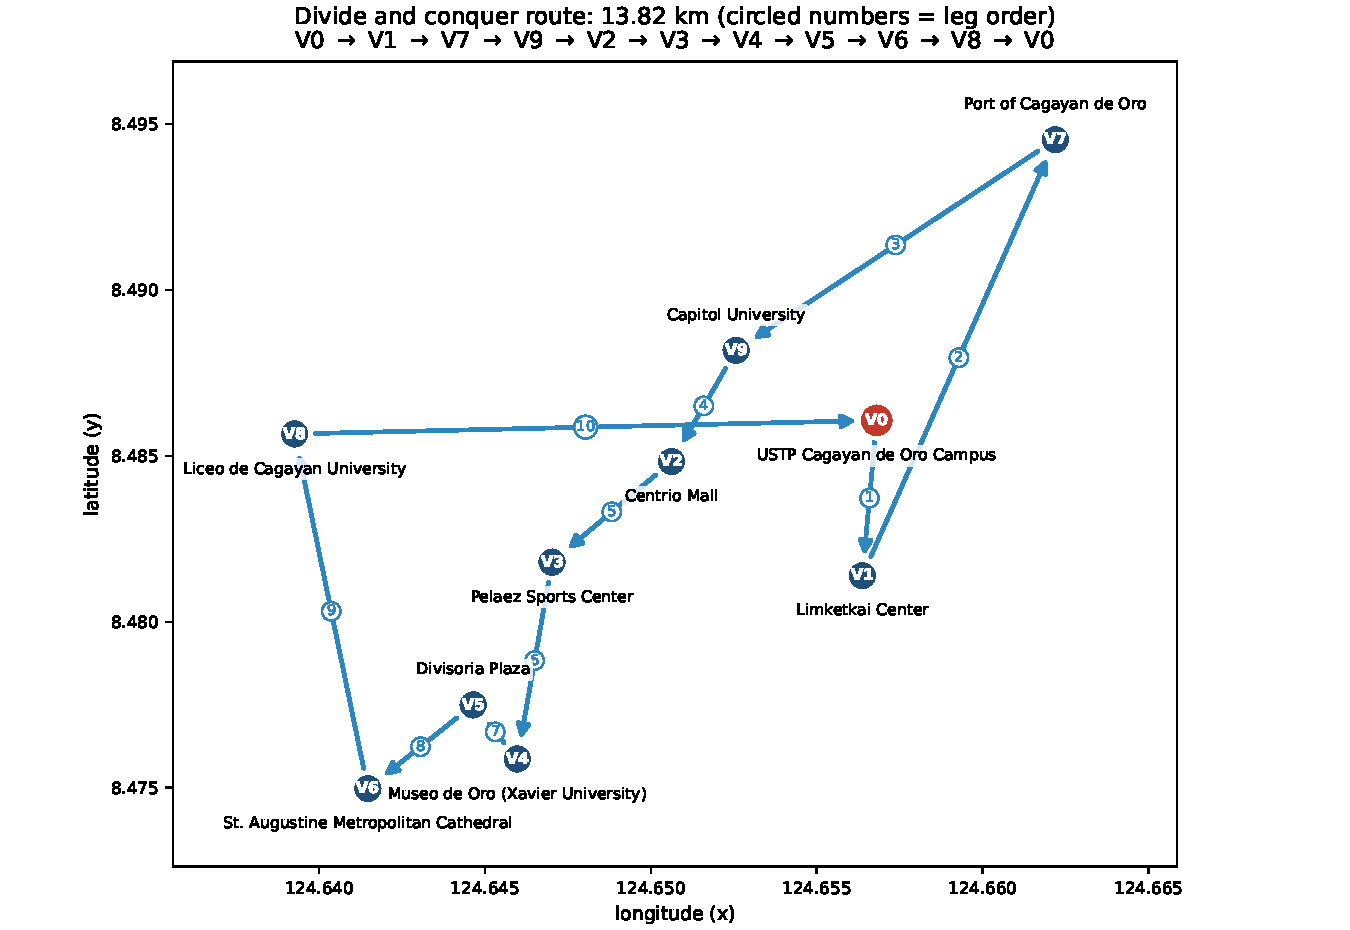
\includegraphics[height=0.86\textheight]{route.pdf}
\end{frame}

\begin{frame}{Verification: Recomputing the Total}
  \centering
  \scriptsize
  \setlength{\tabcolsep}{4pt}
  % AUTO-GENERATED by code/main.py --export-latex. Do not edit; re-run the export instead.
\begin{tabular}{c l l r r}
\toprule
\textbf{Leg} & \textbf{From} & \textbf{To} & \textbf{km} & \textbf{Cumulative} \\
\midrule
1 & V0 USTP Cagayan de Oro Campus & V1 Limketkai Center & 1.09 & 1.09 \\
2 & V1 Limketkai Center & V7 Port of Cagayan de Oro & 2.32 & 3.41 \\
3 & V7 Port of Cagayan de Oro & V9 Capitol University & 1.79 & 5.20 \\
4 & V9 Capitol University & V2 Centrio Mall & 0.58 & 5.78 \\
5 & V2 Centrio Mall & V3 Pelaez Sports Center & 1.18 & 6.96 \\
6 & V3 Pelaez Sports Center & V4 Museo de Oro (Xavier University) & 1.31 & 8.27 \\
7 & V4 Museo de Oro (Xavier University) & V5 Divisoria Plaza & 0.54 & 8.81 \\
8 & V5 Divisoria Plaza & V6 St. Augustine Metropolitan Cathedral & 0.74 & 9.55 \\
9 & V6 St. Augustine Metropolitan Cathedral & V8 Liceo de Cagayan University & 1.65 & 11.20 \\
10 & V8 Liceo de Cagayan University & V0 USTP Cagayan de Oro Campus & 2.62 & 13.82 \\
\midrule
\multicolumn{3}{r}{\textbf{Total}} & \multicolumn{2}{r}{\textbf{13.82 km}} \\
\bottomrule
\end{tabular}


  \medskip
  \footnotesize
  \textbf{Checks (all \DCAllChecks{}):} starts at V0 \textbullet{} returns to V0 \textbullet{}
  \NumVertices{} legs \textbullet{} each location exactly once \textbullet{}
  recomputed \DCRecomputed{} km = reported \DCTotal{} km
\end{frame}

% Suggested time: 1-2 minutes
\section{Conclusion}

\begin{frame}{Interpreting the Route}
  \small
  \begin{itemize}
    \item Meets the objective's constraints: leave USTP, visit each of the 9 landmarks \textbf{exactly once},
          return to USTP, in one loop of \textbf{\DCTotal{} km}.
    \item Nearby places are grouped: the Divisoria cluster V4, V5, V6 is visited consecutively
          (0.54 and 0.74 km).
    \item Driven with the raw one-way distances, the same route is \textbf{13.54 km}; 13.82 km uses the
          averaged, undirected weights of the model.
  \end{itemize}
  \medskip
  \begin{block}{Where the route loses to the optimum}
    \footnotesize
    Only the order inside the cluster differs: ours V3$\to$V4$\to$V5$\to$V6 ($1.31+0.54+0.74 = 2.59$ km),
    optimal V3$\to$V5$\to$V4$\to$V6 ($0.97+0.54+0.87 = 2.38$ km). Merge M2 must add the shortest bridge
    V6--V5, so the edge V6--V4 is never considered. The long leg V8$\to$V0 is \emph{not} the cause:
    the optimal tour uses it too.
  \end{block}
\end{frame}

\begin{frame}{Is It Optimal? No --- and We Can Show It}
  \small
  Exact Held--Karp~\cite{heldkarp1962} on the same graph, used only for comparison:
  \begin{center}
    \OptRoute{} \quad = \textbf{\OptTotal{} km}
  \end{center}
  Our Divide and Conquer route: \textbf{\DCTotal{} km}, i.e.\ \textbf{\DCGap\% above optimal}, so it is an
  \textbf{approximate} solution.
  \medskip

  \centering
  \scriptsize
  % AUTO-GENERATED by code/main.py --export-latex. Do not edit; re-run the export instead.
\begin{tabular}{l r r r r r r r}
\toprule
\textbf{Method} & \textbf{Best} & \textbf{Worst} & \textbf{Mean} & \textbf{Std.} & \textbf{Mean gap} & \textbf{Optimal} & \textbf{ms/run} \\
\midrule
Shortest bridge (paper) & 13.61 & 14.26 & 13.88 & 0.25 & 2.01\% & 6/100 & 0.405 \\
Best splice (variant) & 13.61 & 14.13 & 13.91 & 0.24 & 2.20\% & 17/100 & 0.342 \\
Held--Karp (exact) & 13.61 & 13.61 & 13.61 & 0.00 & 0.00\% & -- & -- \\
\bottomrule
\end{tabular}


  \medskip
  \footnotesize The paper reports 10 runs; we repeated ours over \RunCount{} random seeds. Only \BridgeOptHits{}
  runs happened to be optimal, and the algorithm cannot tell which; only Held--Karp shows it.
\end{frame}

\begin{frame}{Limitations and Improvements}
  \begin{columns}[T]
    \begin{column}{0.48\textwidth}
      \begin{block}{Limitations}
        \small
        \begin{itemize}
          \item Approximate (\DCGap\% above optimal); depends on the seed (\BridgeBest{}--\BridgeWorst{} km
                over \RunCount{} seeds)
          \item Distance only: no traffic or time windows
          \item One-way streets averaged (13.54 km on raw one-way values)
          \item OSRM vs.\ Google Maps: 13.82 vs.\ 14.40 km; optimality is shown for the OSRM matrix only
        \end{itemize}
      \end{block}
    \end{column}
    \begin{column}{0.48\textwidth}
      \begin{block}{Improvements}
        \small
        \begin{itemize}
          \item 2-opt: reversing V4$\to$V5 swaps V3--V4, V5--V6 ($1.31+0.74$) for V3--V5, V4--V6
                ($0.97+0.87$), saving 0.21 km $\Rightarrow$ exactly \OptTotal{} km
          \item Restart with several seeds, keep the best (best of \RunCount{}: \BridgeBest{} km; only
                Held--Karp shows it is optimal)
          \item Best-splice merge: more optimal hits, but no better on average
          \item Travel-time weights from Google Maps
        \end{itemize}
      \end{block}
    \end{column}
  \end{columns}
\end{frame}

\begin{frame}{Conclusion}
  \begin{itemize}
    \item Modelled a downtown Cagayan de Oro tour as a TSP on $K_{\NumVertices}$ with road distances (km).
    \item Implemented Divide and Conquer (Algorithm 2.8), fixing the merge so that it always gives a
          valid Hamiltonian cycle, in $O(n^2)$ time.
    \item Route: \DCRoute{}
    \item Total \textbf{\DCTotal{} km}, verified; \textbf{\DCGap\% above} the optimum of \OptTotal{} km.
    \item Fast and valid, but \textbf{approximate}, not proven optimal.
  \end{itemize}
\end{frame}

\begin{frame}[allowframebreaks]{References}
  \tiny
  \nocite{lunagarcia2024performance, karp1977probabilistic, codingdrills_dc_tsp, morenomaza_dc, osm, googlemaps, luxen2011osrm, hunter2007matplotlib, applegate2006tsp}
  \bibliographystyle{plain}
  \bibliography{dc-tsp-refs}
\end{frame}


\end{document}
